\section{Introduction}
\label{sec:introduction}

The simple recipe of minimizing next-token prediction error at scale has led to large multimodal foundation models (LMs) with remarkably general capabilities~\citep{openai2023gpt4, anil2023gemini, anthropic2024claude3}.
Importantly, these capabilities come in two flavors: (i) the ability to produce outputs of high quality from a short and often underspecified prompt (\eg writing an essay about a novel topic), and (ii) the ability to learn new patterns and imitate algorithms \emph{in context}~\citep{reid2024gemini, mirchandani2023large}.
Both types of capabilities demonstrate that LMs
can manipulate learned knowledge and respond to new information in flexible and non-trivial ways.
These capabilities, both necessary for reasoning and decision-making, have led to the recent surge of using LMs as agents by sampling an action from the model~\citep{mirchandani2023large, dipalo2024keypoint}.

While LMs have been shown to be able to perform non-trivial reasoning and decision-making in some domains~\citep{ huang2022language,yao2023react,romera2024mathematical}, there are also many negative results where LMs fail to perform decision-making tasks that are very simple for humans, even when LMs arguably possess great factual knowledge of the task.
For example, LMs struggle to play legal moves, let alone beat amateur humans, in chess~\citep{carlini2023playing}.
At the same time, state-of-the-art LMs have detailed expert knowledge of chess when queried in natural language. But this \emph{declarative} knowledge fails to translate into effective decision-making, \ie ``know-how''~\citep{ryle1949concept}.
This ``knowing-doing gap'' is also observed in the recently released BALROG benchmark~\citep{paglieri2025balrog}, which evaluates zero-shot capabilities (\ie without expert demonstrations) of state-of-the-art LMs on interactive decision-making tasks in the long time horizon setting: 5 game environments from Baby AI~\citep{chevalier2019babyai} to Nethack~\citep{kuttler2020nethack}.
Overall, \citet{paglieri2025balrog} find that ``models struggle significantly with more challenging tasks'' and highlight few- and many-shot evaluation as an important potential solution.
Our benchmark (developed concurrently) addresses exactly this gap by covering the full range from zero-shot to many-shot evaluation.

\begin{figure*}[t]
    \begin{center}
        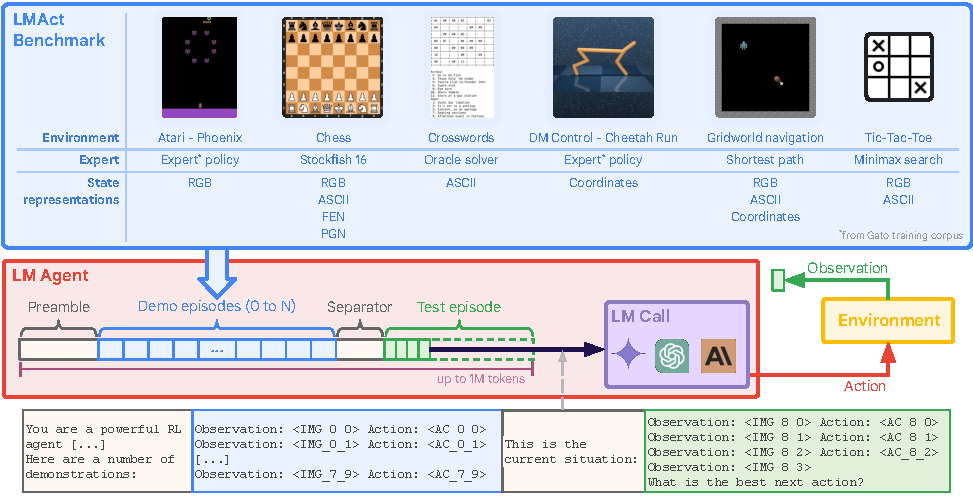
\includegraphics[width=0.8\textwidth]{figures/LMActOverviewFigure.pdf}
    \end{center}
    \vspace{-8pt}
    \caption{
        LMAct overview.
        Our multimodal benchmark consists of six decision-making tasks that come with an expert policy and potentially multiple state representations.
        For evaluation, LM performance is measured on test episodes with unseen initial states.
        LMs are conditioned on a generic decision-making preamble (fixed across all tasks), followed by $0$ to $N$ demonstration episodes, and a separator that indicates the start of the current episode ($N$ can be up to $512$, with up to $100$ steps per episode, both depending on the task. The maximum context length is $1$M tokens).
        In each step of the test episode an action is generated by the LM's predicted continuation of the context.
        \ificlr
        The resulting environment interaction produces the next observation that is added to the previous state action pairs.
        \else
        The resulting environment interaction produces the next observation that is added to the growing context of state action pairs.
        \fi
    }
    \vspace{-4pt}
    \label{fig:overview}
\end{figure*}

The general question arising from these results is whether LMs in principle have the capabilities to solve interactive decision-making tasks but misunderstand the ``out-of-distribution'' specification given by the zero-shot prompt or a few examples, or whether the problem is more deeply rooted.
Accordingly, our paper focuses on whether conditioning on a \emph{large} number of expert demonstrations (state-action trajectories) helps unlock the decision-making capability of pretrained LMs.
In doing so, we test the multimodal in-context learning capabilities of modern LMs at their limits, with contexts that are up to a million tokens long (with thousands of output tokens).
Our main research question is:
\begin{quote}
    Can state-of-the-art LMs learn to act in dynamic environments by generalizing from \emph{large} numbers of \emph{multimodal} in-context expert demonstrations?
\end{quote}

\paragraph{Main Contributions}

See \Cref{fig:overview} for our tasks and methodology.
\ificlr
Our key contributions are:
\else
We make the following key contributions:
\fi

\begin{itemize}
    \item We conduct a comprehensive empirical evaluation of the multimodal in-context imitation learning capabilities of state-of-the-art LMs (\claude, \flash, \pro, \expflash, \gpt, \mini, \preview, and \oone) on a battery of interactive, potentially long-horizon, tasks: playing tic-tac-toe, chess, and Atari, navigating grid worlds, solving crosswords, and a DM~Control task.
    \item We show that --- even when optimizing the prompt (number of demonstrations, chain-of-thought prompting, \etc) for each model and task --- frontier LMs fail to reach expert performance on Atari, chess, and DM Control.
    Some models approach expert performance on crosswords, grid world, and tic-tac-toe.
    All models beat the random action baselines except on Atari.
    \item We vary the number of expert demonstration episodes in the context from $0$ up to $512$ (the limit depends on the model and the task) and find that performance is mostly independent of the number of demonstrations. In some cases we observe strong in-context learning.
    \item We run a control experiment where LLM agents need to replay the single demonstration episode in the context, where all models except for \mini{} perform well.
    \item We open-source \ificlr
    LMAct,
    \else\fi our in-context imitation learning benchmark that covers the zero-, few-, and many-shot regime in a unified manner, including all expert demonstrations and evaluation code at
    \url{https://github.com/google-deepmind/lm_act}.
\end{itemize}

